\section{Methods and Materials}
\label{methods}
\subsection{Ethical Clearance}
\label{methods_ethical}
\subsubsection*{Data Considerations}
\subsubsection*{Application Details}

\subsection{Software Design}
\label{methods_softwaredesign}
\subsubsection{Requirements}
\subsubsection{Tools}
\paragraph{Git and Github}
(\url{http://git-scm.com/}),
(\url{http://www.github.com/})

Git is a distributed version control system (VCS) which tracks changes
to source code (often amongst multiple developers) and keeps a complete history
of changes. This is invaluable when a change in code occurs that results in a critical
bug. Versions can be compared to find the change that introduced the bug, and production
code can be reverted if need be \cite{scott_chacon_pro_2009}.

Git can be hosted anywhere, however Github is a popular 

\paragraph{Ruby on Rails}
(\url{http://www.rubyonrails.org/})

Ruby on Rails is a popular open source framework for developing web applications\cite{bachle_ruby_2007}.

% TODO Complete Rails section

\paragraph{Heroku}
(\url{http://www.heroku.com/})

% TODO Complete Heroku section

\paragraph{Highcharts}
(\url{http://www.highcharts.com/})

Highcharts is a Javascript 
% TODO Complete Highcharts section

\paragraph{Twitter Bootstrap}
(\url{http://twitter.github.com/bootstrap})

Twitter Bootstrap is a set of default styles for websites and web applications, provided as open-source by Twitter. Using Twitter Bootstrap rapidly speeds up theming of a web application with default looks for navigation, buttons, text and layout.


Compare the following pages with and without Twitter Bootstrap default styles added:
\begin{figure}[h!]
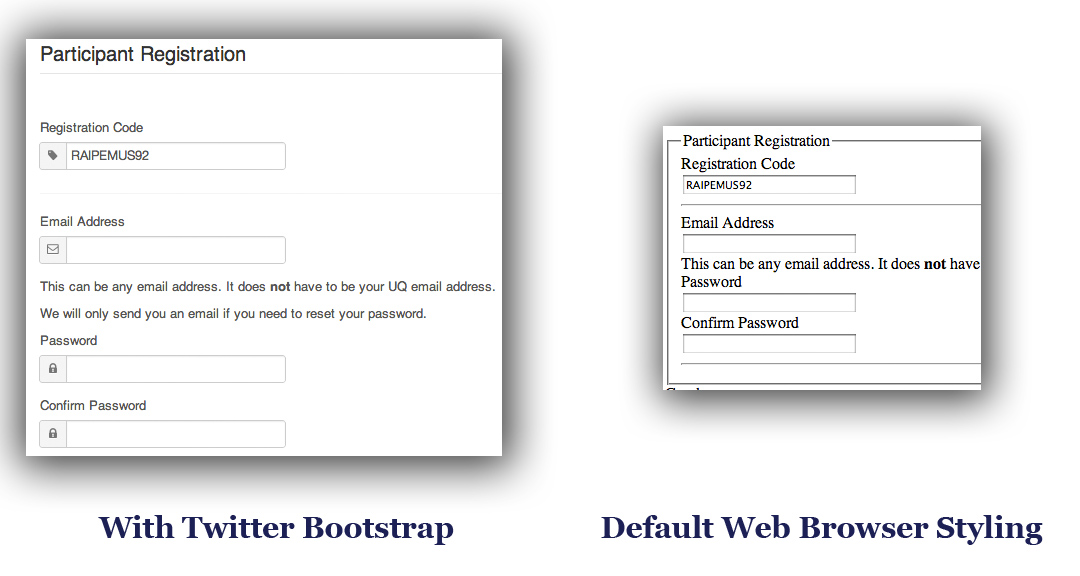
\includegraphics[width=120mm]{img/twitterbootstrap.jpg}
\caption{Comparison of a page with no styling and Twitter Bootstrap default styling}
\end{figure}

More significantly, Twitter Bootstrap offers a 'responsive' layout 
system which provides a reduced screen size (ie. smartphone) layout
 with little to no extra work on the part of the developer. This 
 means a smartphone version of the web application could be designed
  at the same time. Twitter Bootstrap was also chosen for this reason.
\subsubsection{Data Entry}
\subsubsection{Screen Mockups}
\subsubsection{Spaced Repetition Algorithm}
\subsubsection{Data storage, formatting and output}

\subsection{Data Analysis and Prediction}
\subsubsection{R Programming Language}
\subsubsection{Usage Data}
\subsubsection{Forgetting Curves}
\subsubsection{Prediction of Recall}